\documentclass[compress]{beamer}

\usetheme{Warsaw}

\usepackage[utf8]{inputenc}
\usepackage[russian]{babel}
\usepackage{cmap}

\usefonttheme{professionalfonts}
\usepackage{graphicx}
\usepackage{psfrag}
\beamertemplatenavigationsymbolsempty 
\DeclareMathOperator{\sign}{sign}

\author{Павел Филонов \\ \href{mailto:filonovpv@gmail.com}{filonovpv@gmail.com}}
\title{Введение в машинное обучение}
\subtitle{Задачи классификации и регрессии}

\begin{document}
\begin{frame}
    \titlepage
\end{frame}
\begin{frame}{Содержание}
  \tableofcontents
\end{frame}
\section{Основные понятия и обозначения}
\subsection{Постановка задачи машинного обучения}
\begin{frame}
Пусть
    \begin{itemize}
        \item $X$ --- множество объектов (objects);
        \item $Y$ --- множество ответов (targets);
        \item $y: X \rightarrow Y$ --- неизвестная зависимость (target function).
    \end{itemize}
    {\bf Дано:}
    \begin{itemize}
        \item $\{x_1, \dots, x_l\} \subset X$ --- обучающая выборка (training sample);
        \item $y_i = y(x_i),~ i=1,\dots, l$ --- известные ответы (known targets).
    \end{itemize}
    {\bf Найти:}
    $a: X \rightarrow Y$ --- алгоритм, решающую функцию (decision function), приближающую $y$ на всём множестве $X$.


Весь курс машинного обучения--- это конкретизация:
    \begin{itemize}
        \item как задаются объекты и какими могут быть ответы;
        \item в каком смысле <<$a$ приближает $y$>>;
        \item как строить функцию $a$.
    \end{itemize}

% Приведенная задача --- представляет собой центральную проблему, которая красной нитью проходит через весь курс.
\end{frame}

\subsection{Представление объектов. Признаковое описание}
\begin{frame}
$f_j: X \rightarrow D_j, j=1,\dots,n$ --- принаки объектов (features).

Типы признаков:
\begin{itemize}
    \item $D_j = \{0, 1\}$ --- бинарный признак;
    \item $|D_j| < \infty$ --- номинальный признак;
    \item $|D_j| < \infty, ~ D_j - \text{упорядочено}$ --- порядковый признак;
    \item $D_j = \mathbb{R}$ --- количественный признак.
\end{itemize}

Вектор $\left(f_1(x),\dots,f_n(x)\right)$ --- признаковое описание объекта $x$.

Матрица <<объекты-признаки>> (feature matrix)
$$
F = ||f_j(x_i)||_{l \times n} = \begin{pmatrix}
    f_1(x_1) & \cdots & f_n(x_1) \\
    \vdots   & \ddots &   \vdots \\
    f_1(x_l) & \cdots & f_n(x_l) \\
    \end{pmatrix}
$$
\end{frame}

\subsection{Представление ответов. Типы задач}
\begin{frame}{Представление ответов. Типы задач}
    
    {\bf Задача классификации} (classification):
    \begin{itemize}
        \item $Y = \{-1, +1\}$ --- бинарная классификация;
        \item $Y = \{1, \dots, M\}$ --- на $M$ непересекающихся классов;
        \item $Y = \{0, 1\}^M$ --- на $M$ классов, которые могут пересекаться.
    \end{itemize}
    \vfill

    {\bf Задача восстановления регресии} (regression):
    \begin{itemize}
        \item $Y = \mathbb{R}$ --- одномерная;
        \item $Y = \mathbb{R}^m, ~ m > 1$ --- многомерная (multivariate).
    \end{itemize}
    \vfill

    {\bf Задача ранжирования} (ranking)
    \begin{itemize}
        \item $Y$ --- конечное упорядоченное множество.
    \end{itemize}
\end{frame}
\begin{frame}{Задача классификации цветков ириса [Фишер, 1936]}
    \footnotesize $n = 4$ количественный признака, $|Y| = 3$ класса, объем выборки $l = 150$.
    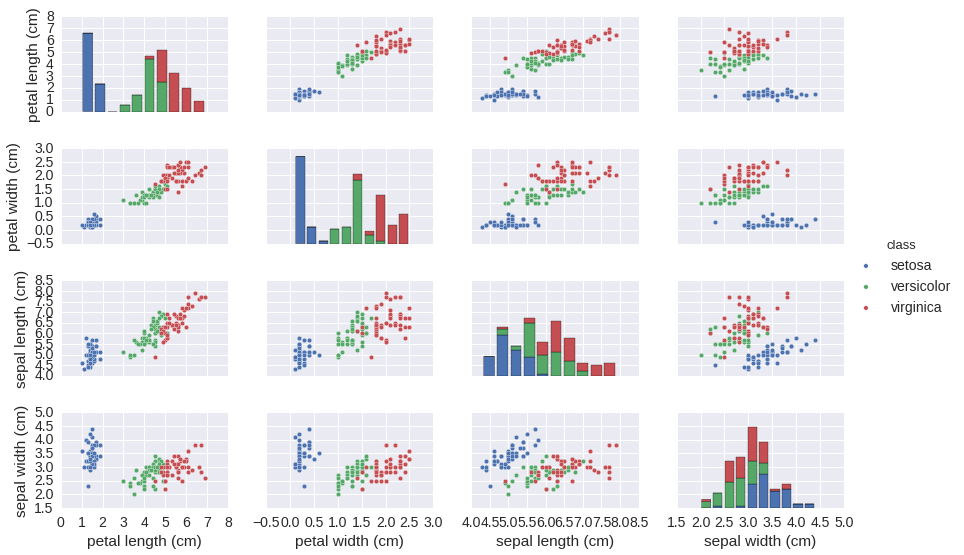
\includegraphics[width=\linewidth]{fig/iris.png}
\end{frame}
\begin{frame}{Задача оценки стоимости жилья в Бостоне}
    \begin{center}
        $n = 13, Y= \mathbb{R}, l = 506$
        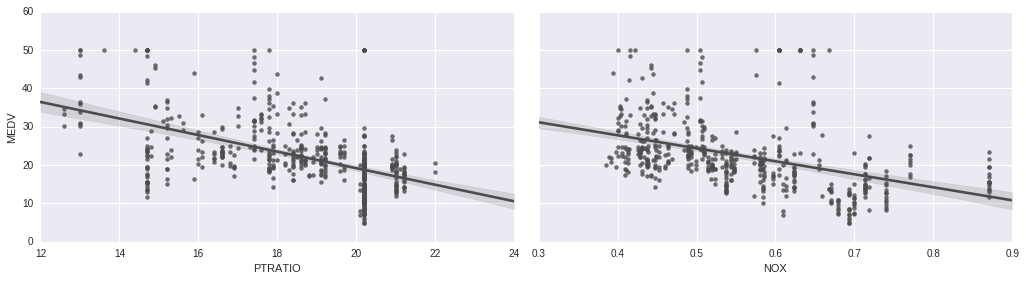
\includegraphics[width=\linewidth]{fig/boston1.png}
        \\
        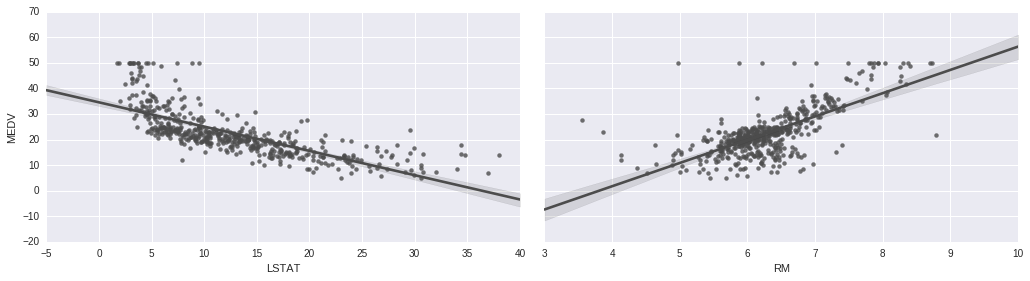
\includegraphics[width=\linewidth]{fig/boston2.png}
    \end{center} 
\end{frame}

\subsection{Модели и методы обучения}
\begin{frame}{Модель алгоритмов}
Модель (predictive model) --- парметрическое семейство функций
$$
    A = \{g(x, \theta) ~|~ \theta \in \Theta\},
$$
где $g : X \times \Theta \rightarrow Y$ --- фиксированная функция,\\
$\Theta$ --- множество допустимых значений параметра $\theta$.

{\bf Пример.}
Линейная модель с вектором параметров $\theta = (\theta_1,\dots,\theta_n), \Theta = \mathbb{R}^n$:
$$
    g(x, \theta) = \sum\limits_{j=1}^{n}\theta_j f_j(x) \text{--- для регресии и ранжирования, $Y = \mathbb{R}$};
$$
$$
    g(x, \theta) = \sign\sum\limits_{j=1}^{n}\theta_j f_j(x) \text{--- для классификации, $Y = \{-1, +1\}$}.
$$
\end{frame}

% \begin{frame}{Машинное обучение ранжированию <<Интернет-математика 2009>>}

% \end{frame}
\section{Функция потерь}
\subsection{Пример 1}
\begin{frame}
\end{frame}
\subsection{Пример 2}
\begin{frame}
\end{frame}
\end{document}